\section{Fiber Bragg Grating technology}

Fiber Bragg Grating is a type of selective filter that reflects light signals at a specific wavelength known as the Bragg wavelength (see Figure 1). A bare FBG inscribed into the fiber core is temperature and strain sensitive.
We can measure RH instead of strain by applying a hygroscopic material (for example, polyimide) to the cladding. The Bragg wavelength shift becomes a superposition of temperature and humidity effects in this case (see equation (see equation \ref{eqn:FBG}) \cite{Kronenberg:02}. 
                            %\newpage
                             \begin{equation}\label{eqn:FBG}
                            %\large
                                    \frac{\Delta\lambda_{B}}{\lambda_{B}}=\Delta TS_{T}+\Delta RHS_{RH}
                            \end{equation}
                            $\lambda_{B}$ - Bragg wavelength, $S_{RH/T}$ - sensitivity  coefficients for RH and temperature, respectively. \newline
In order to measure RH, it’s crucial to have precise temperature readouts in the vicinity of the coated FBG. Otherwise, the actual RH readout may be dominated by uncertainty or just the inaccurate temperature measurement.

\begin{figure}[!h]
\centering
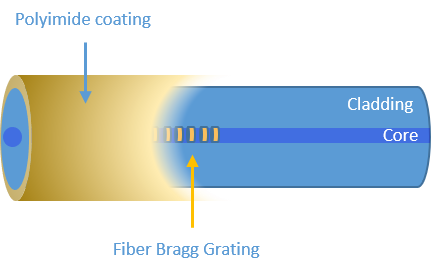
\includegraphics[width=0.4\columnwidth]{Chapter6/images/Picture1.png}
\caption{Hygrometer (Temperature and humidity sensitive FBG inscribed into the same fiber)}
\label{fig_single_photo}
\end{figure}
\section{Evaluation and measurement setup}
A few different humidity sensors have been tested and their performance evaluated. The use of capacitive sensors remains one of the cheapest and easily available solutions for a distributed humidity measurement system. 


\section{Results}


\subsection{Characterization of RH FOS}

\begin{figure}[!h]
\centering
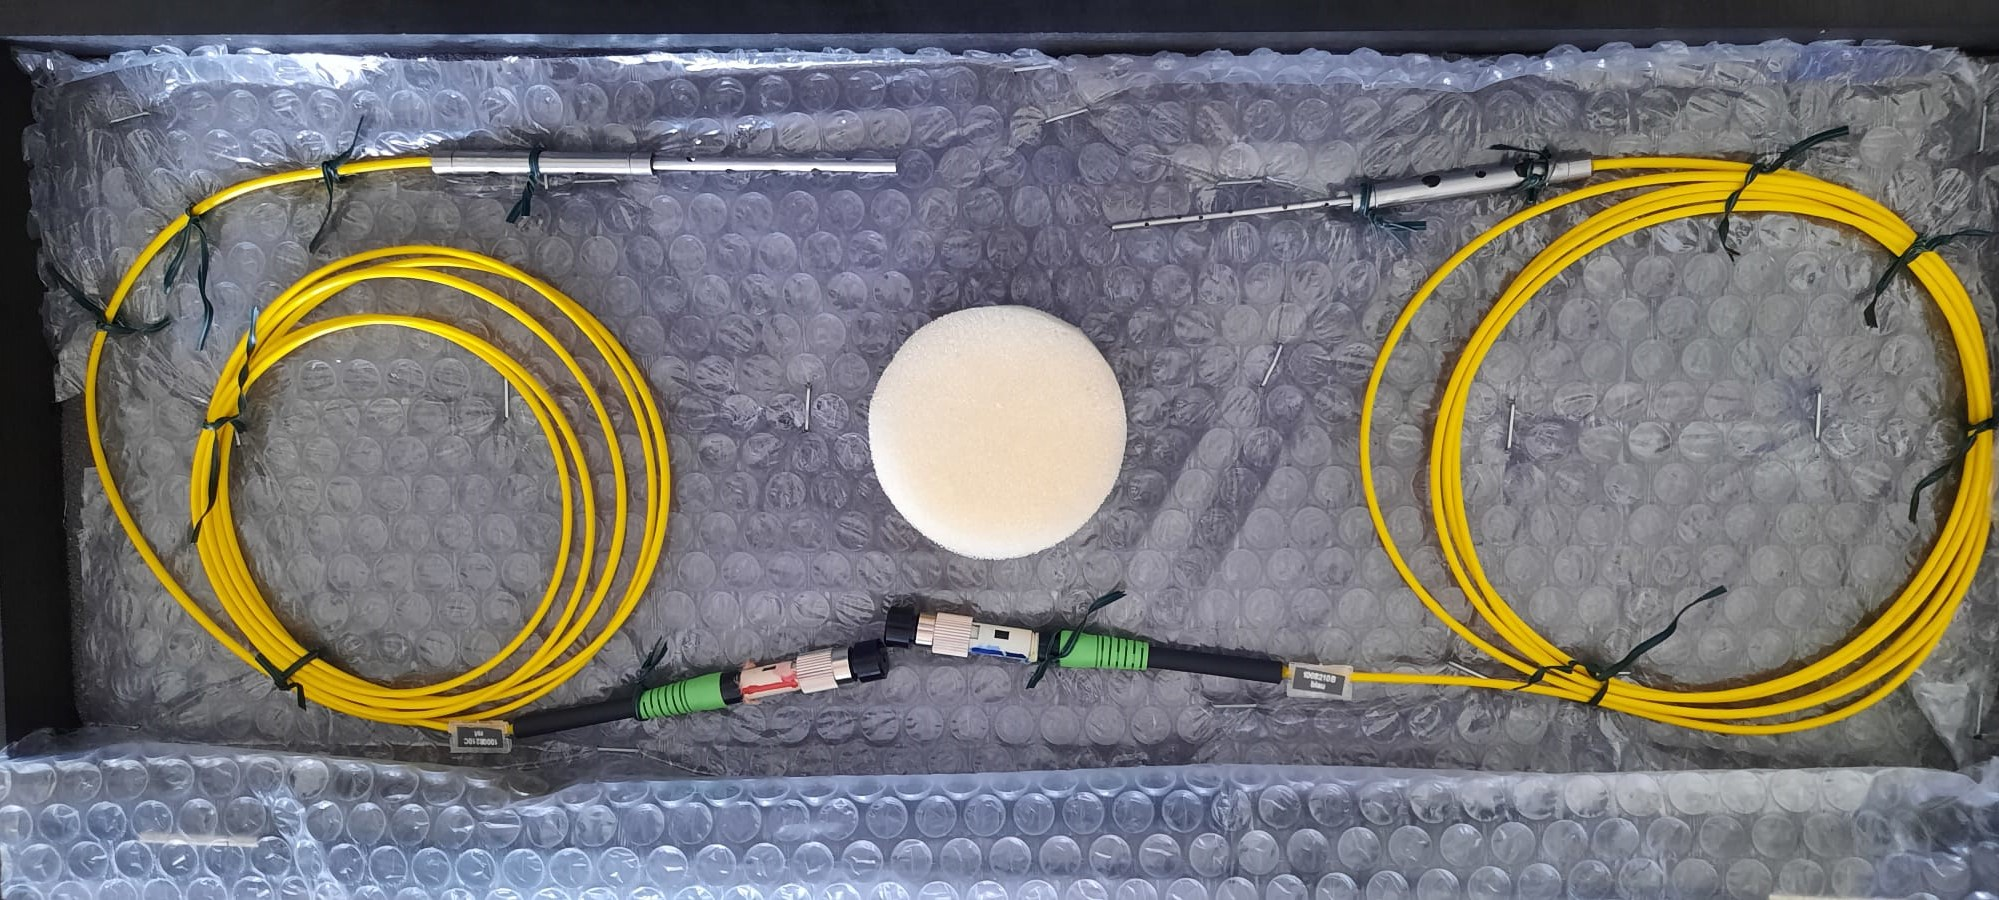
\includegraphics[width=0.65\columnwidth]{Chapter6/images/single1.jpeg}
\caption{Hygrometer (temperature and humidity sensitive FBG inscribed into the same fiber)}
\label{fig_single_photo}
\end{figure}

\begin{figure}[!h]
\centering
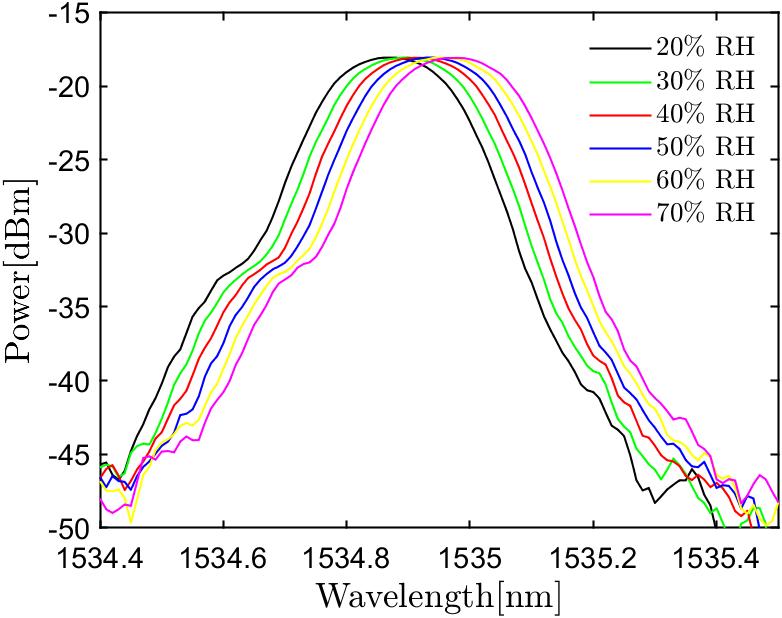
\includegraphics[width=0.6\columnwidth]{Chapter6/images/rh.png}
\caption{Humidity induced Bragg wavelength shift for the single RH+T sensor}
\label{fig_single_wavelength}
\end{figure}


\begin{figure}[!h]
\centering
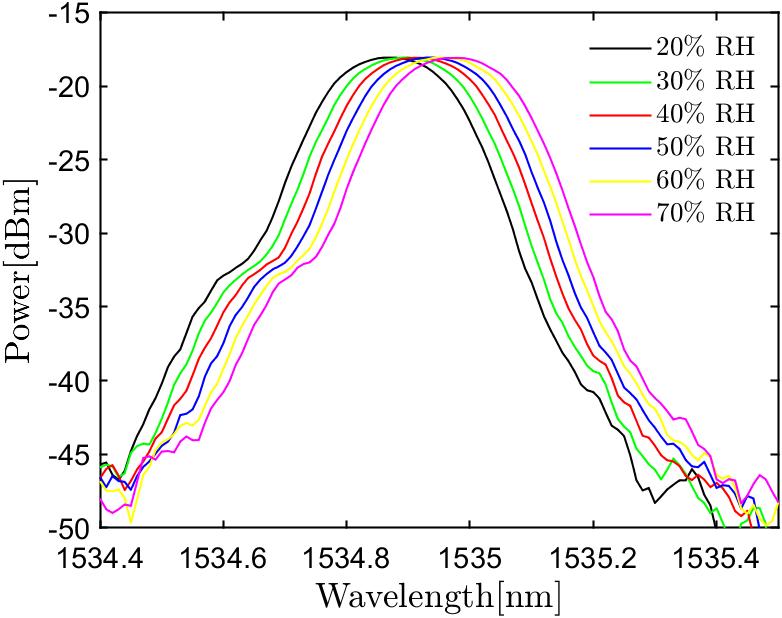
\includegraphics[width=0.6\columnwidth]{Chapter6/images/rh.png}
\caption{Humidity induced Bragg wavelength shift for the hygrometer}
\label{fig_single_wavelength}
\end{figure}


\begin{figure}[!h]
\centering
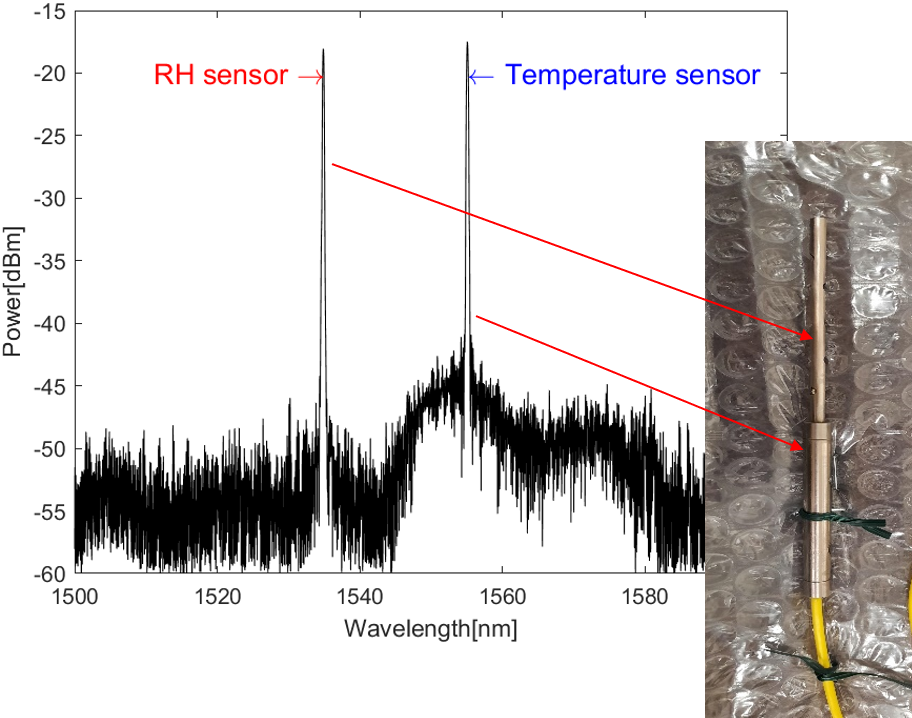
\includegraphics[width=0.6\columnwidth]{Chapter6/images/hygr.png}
\caption{Hysteresis}
\label{fig_hygrometer1}
\end{figure}


\begin{figure}[!h]
\centering
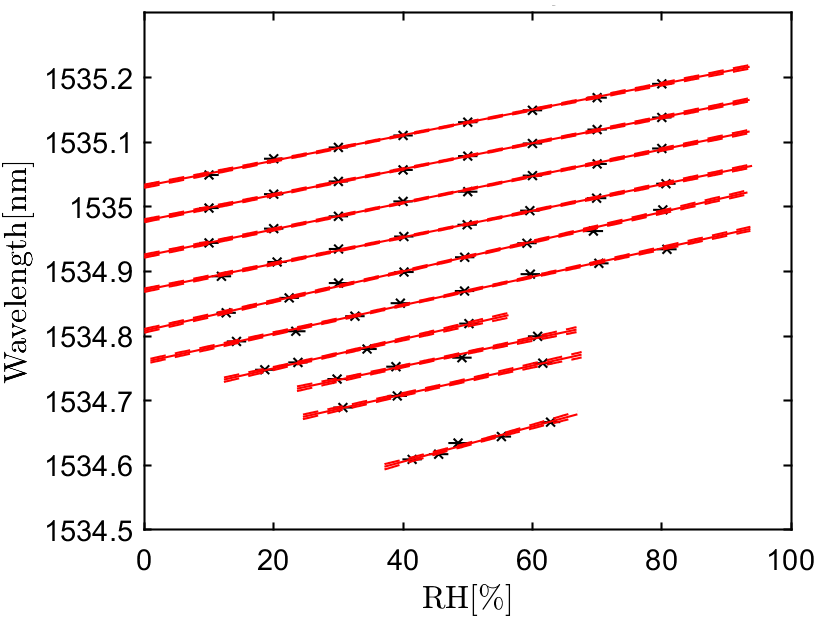
\includegraphics[width=0.6\columnwidth]{Chapter6/images/RHS.png}
\caption{Calibration curves for the hygrometer}
\label{fig_single_calibration}
\end{figure}


\begin{figure}[!h]
\centering
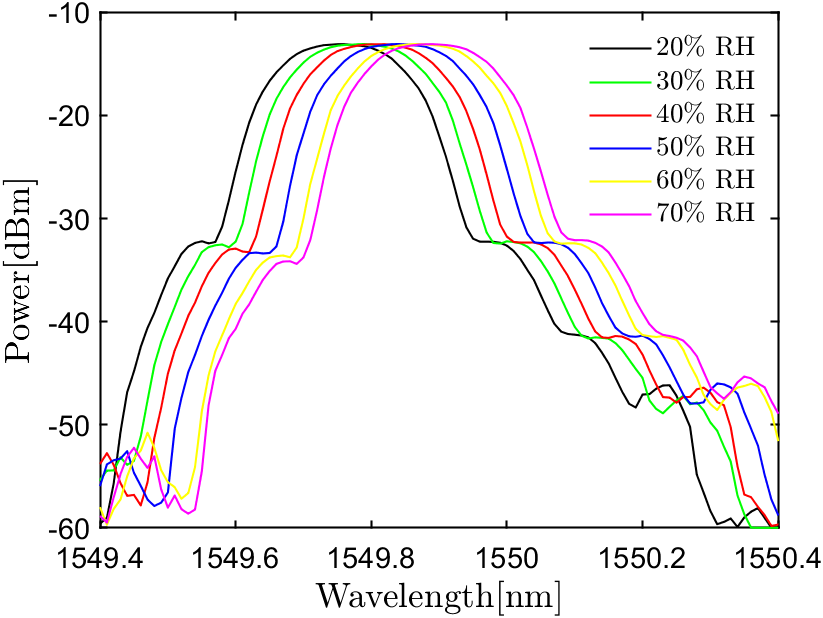
\includegraphics[width=0.6\columnwidth]{Chapter6/images/rh_array2.png}
\caption{Humidity induced Bragg wavelength shift for the sensors array}
\label{fig_single_calibration}
\end{figure}

\subsection{Calibration}

\begin{figure}[!h]
\centering
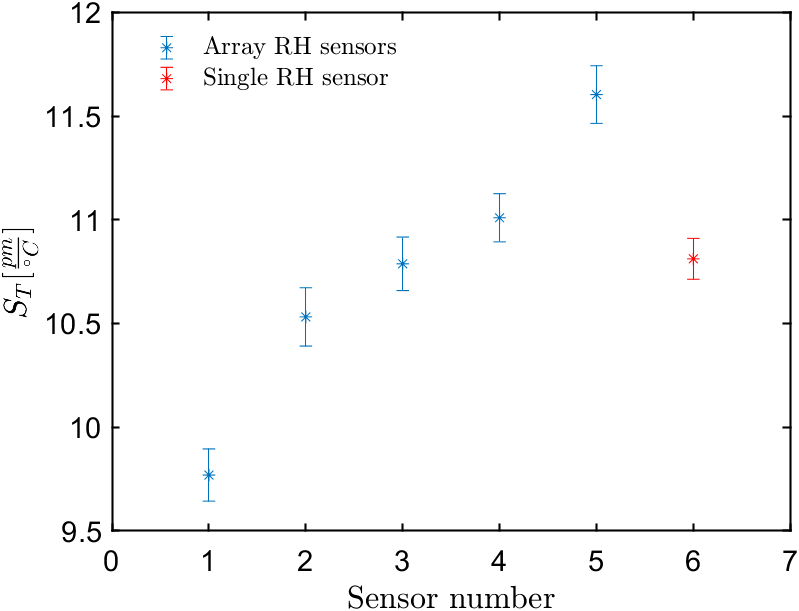
\includegraphics[width=0.6\columnwidth]{Chapter6/images/comp.png}
\caption{Hysteresis}
\label{fig_calibration}
\end{figure}


\begin{figure}[!h]
\centering
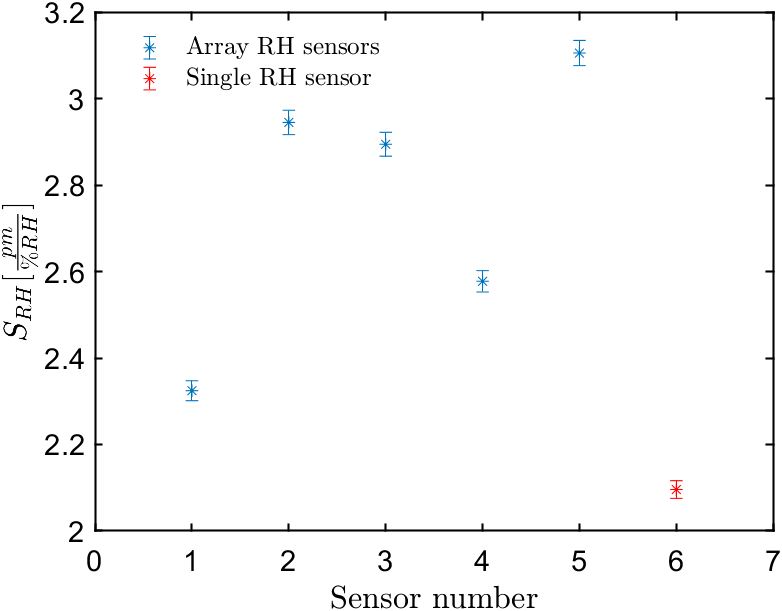
\includegraphics[width=0.6\columnwidth]{Chapter6/images/comp1.png}
\caption{Hysteresis}
\label{fig_calibration1}
\end{figure}





\subsection{Time response}

\begin{figure}[!h]
\centering
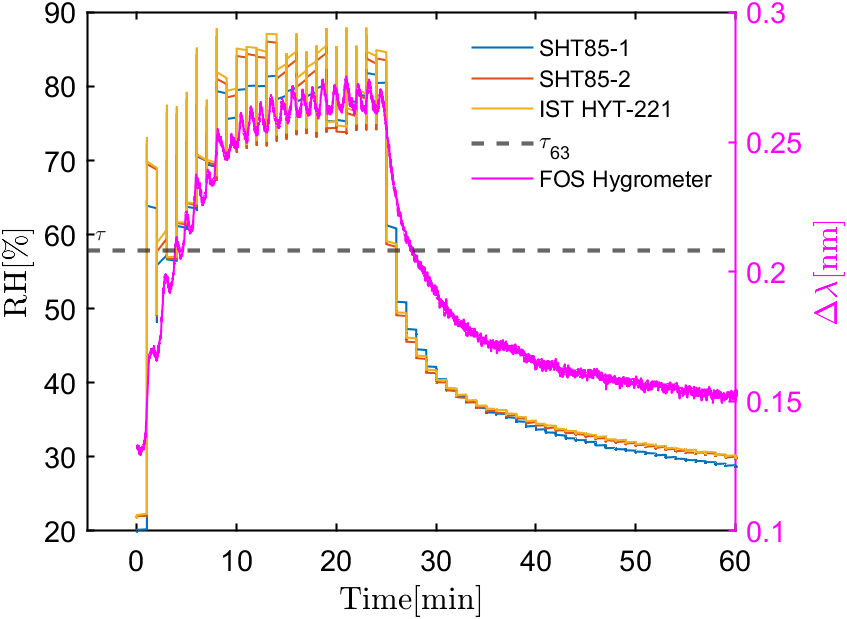
\includegraphics[width=0.6\columnwidth]{Chapter6/images/20responseRH.png}
\caption{Time response of sensors}
\label{fig_time_response}
\end{figure}

\begin{figure}[!h]
\centering
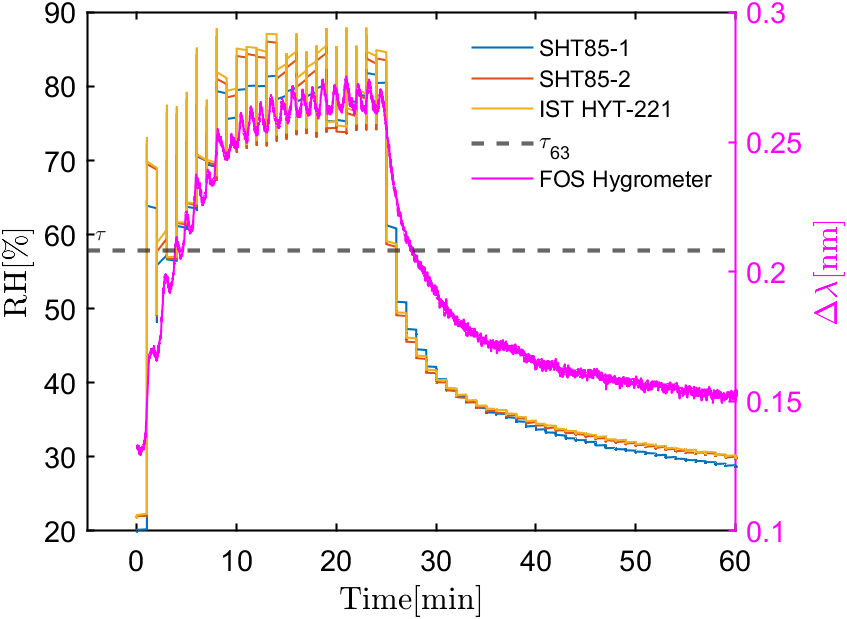
\includegraphics[width=0.6\columnwidth]{Chapter6/images/20responseRH.png}
\caption{Time response of sensors}
\label{fig_time_response}
\end{figure}


\subsection{Hysteresis}

\begin{figure}[!h]
\centering
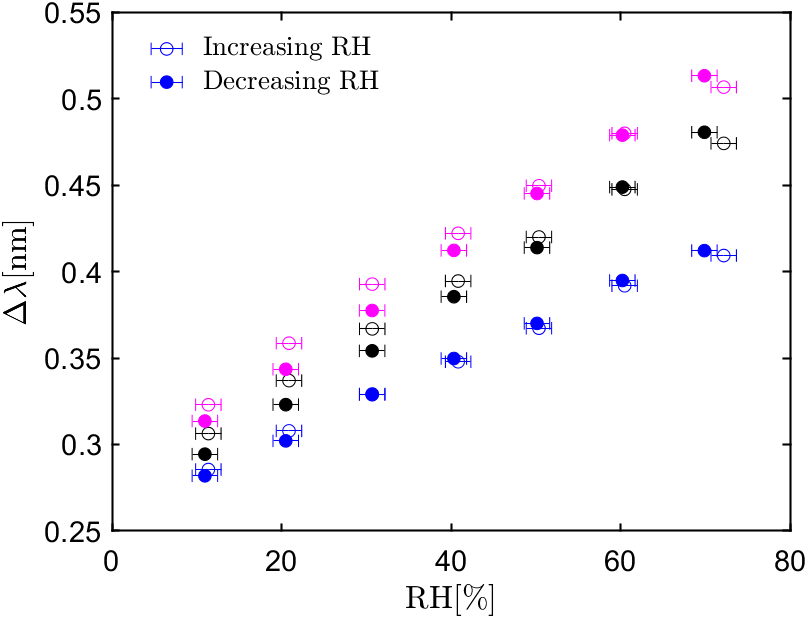
\includegraphics[width=0.6\columnwidth]{Chapter6/images/25_RHS.png}
\caption{Hysteresis}
\label{fig_hysteresis}
\end{figure}

\begin{figure}[!h]
\centering
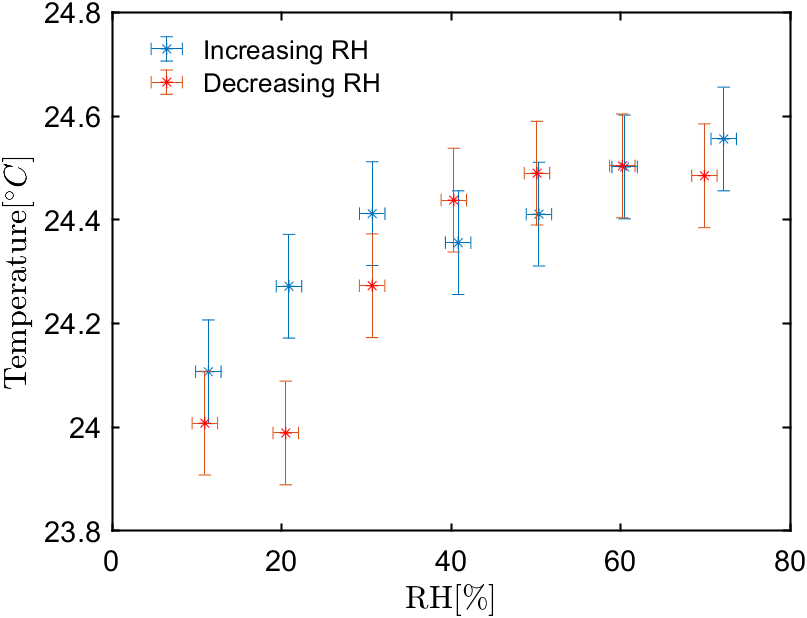
\includegraphics[width=0.6\columnwidth]{Chapter6/images/25_RHST.png}
\caption{Hysteresis}
\label{fig_hysteresis2}
\end{figure}



\subsection{Repeatability}


\begin{figure}[!h]
\centering
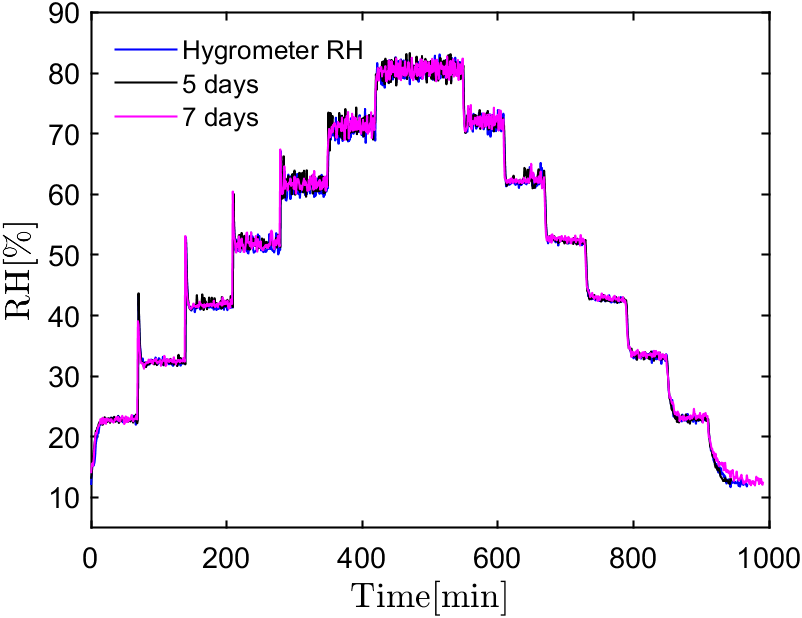
\includegraphics[width=0.6\columnwidth]{Chapter6/images/repeat.png}
\caption{Repeatability}
\label{fig_repeatability}
\end{figure}



\subsection{Conclusions}


\begin{figure}[!h]
\centering
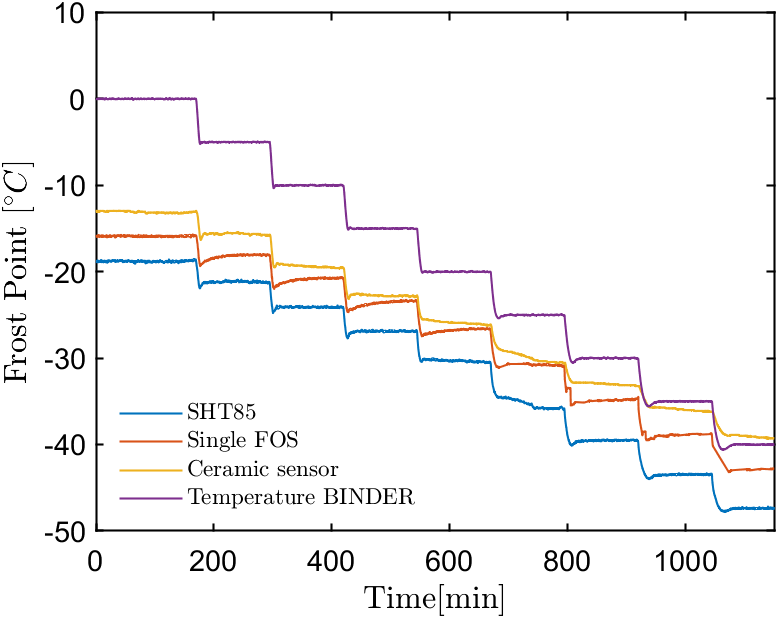
\includegraphics[width=0.6\columnwidth]{Chapter6/images/DPCPercent.png}
\caption{Comparison}
\label{fig_comparison}
\end{figure}

\begin{figure}[!h]
\centering
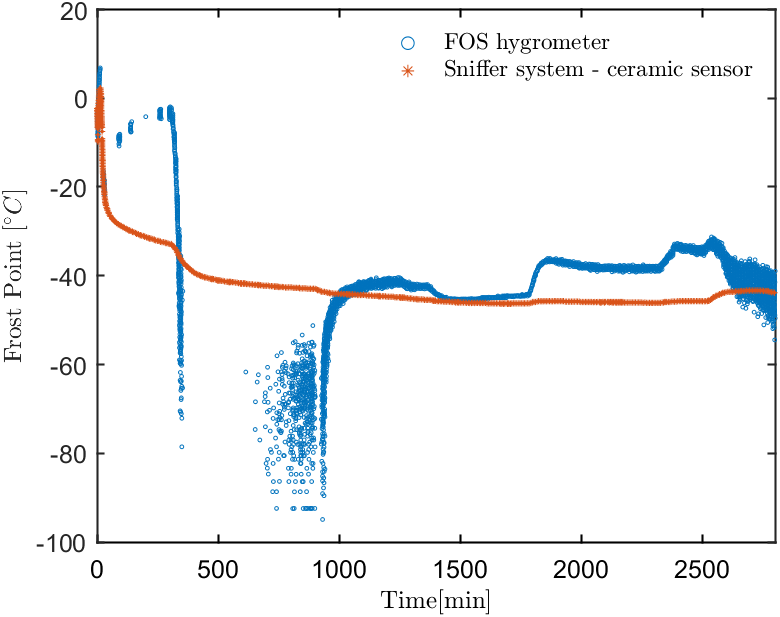
\includegraphics[width=0.6\columnwidth]{Chapter6/images/FOS_performance.png}
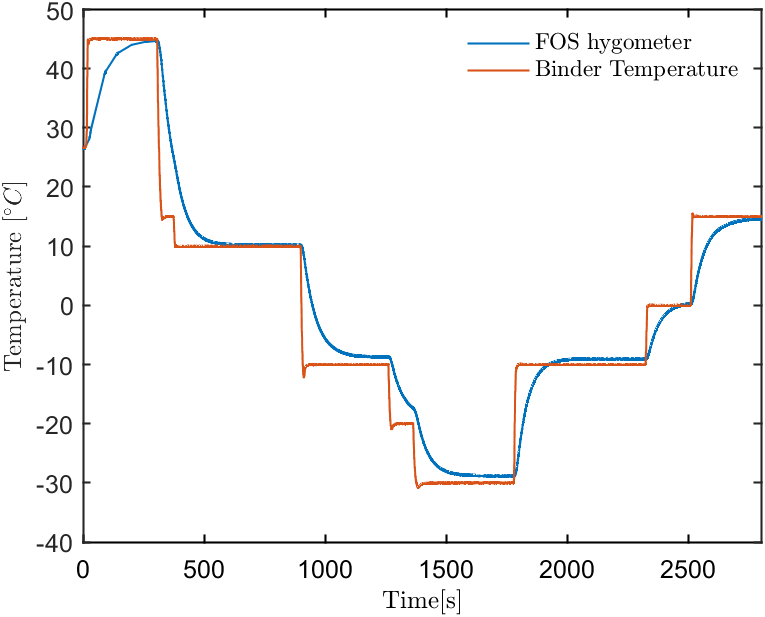
\includegraphics[width=0.6\columnwidth]{Chapter6/images/FOS_performance_T.png}
\caption{Comparison}
\label{fig_comparison}
\end{figure}
